
\documentclass[preview,convert,convert={outext=.png,command=\unexpanded{pdftocairo -r 600 -png \infile}}]{standalone}
\usepackage{graphicx}
\usepackage{subfig}
\graphicspath{{/home/ming/academic/tools/latex2word/tests/en/figures}}
\begin{document}
\thispagestyle{empty}
\begin{figure}[htbp]
    \centering
    \subfloat[]{
        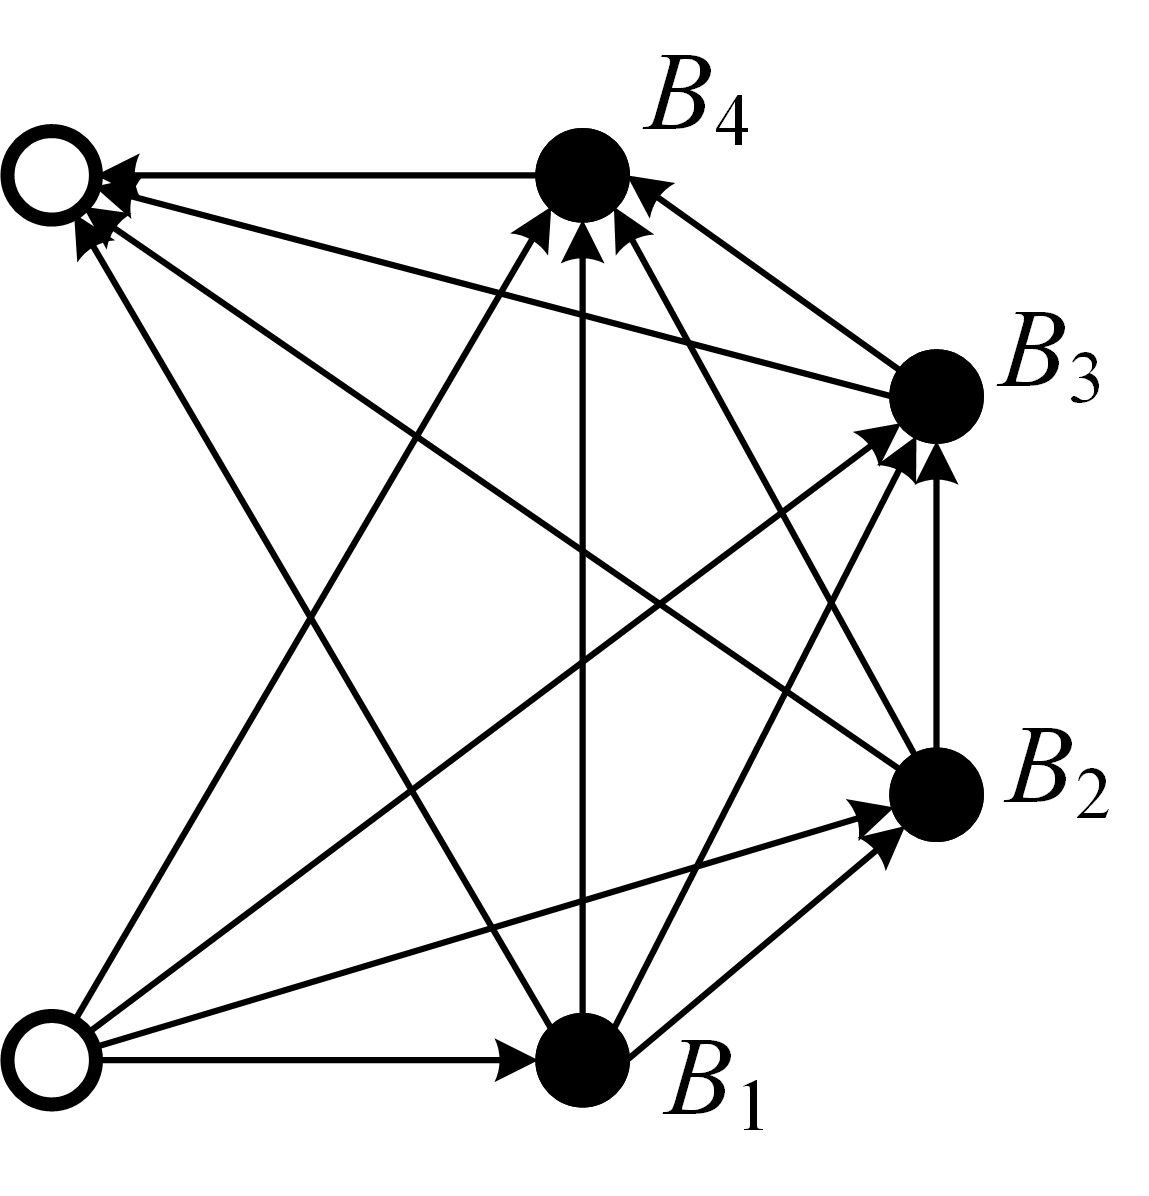
\includegraphics[width=0.31\linewidth]{direct-graph-he.png}
    }\label{fig:direct-graph-he}
    \subfloat[]{
        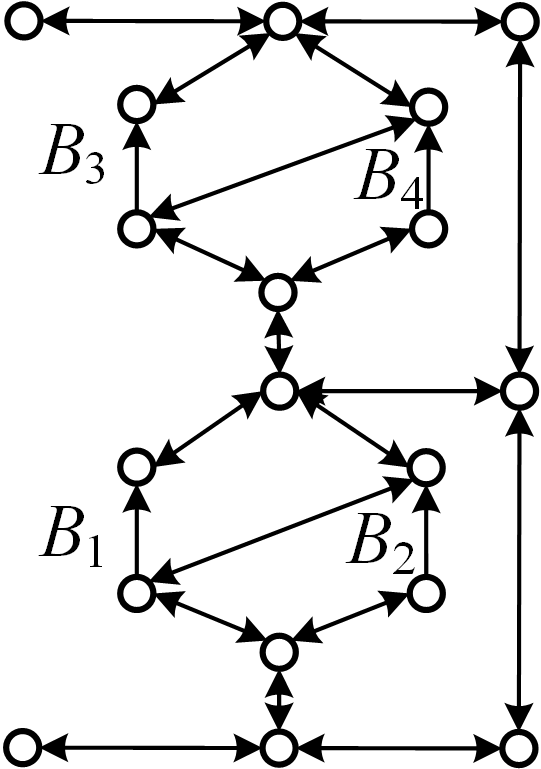
\includegraphics[width=0.23\linewidth]{direct-graph-xu.png}
    }\label{fig:direct-graph-xu}
    \subfloat[]{
        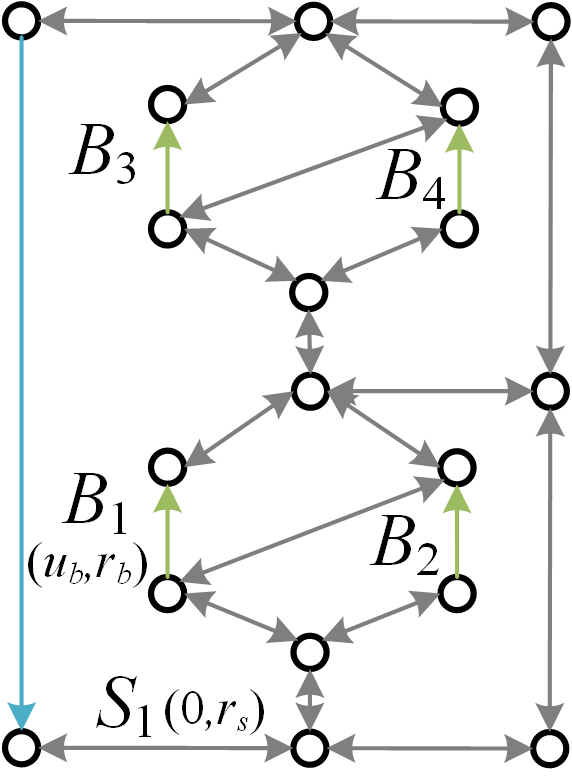
\includegraphics[width=0.24\linewidth]{direct-graph-my.png}
    }\label{fig:direct-graph-my}
    \\
    \subfloat[]{
        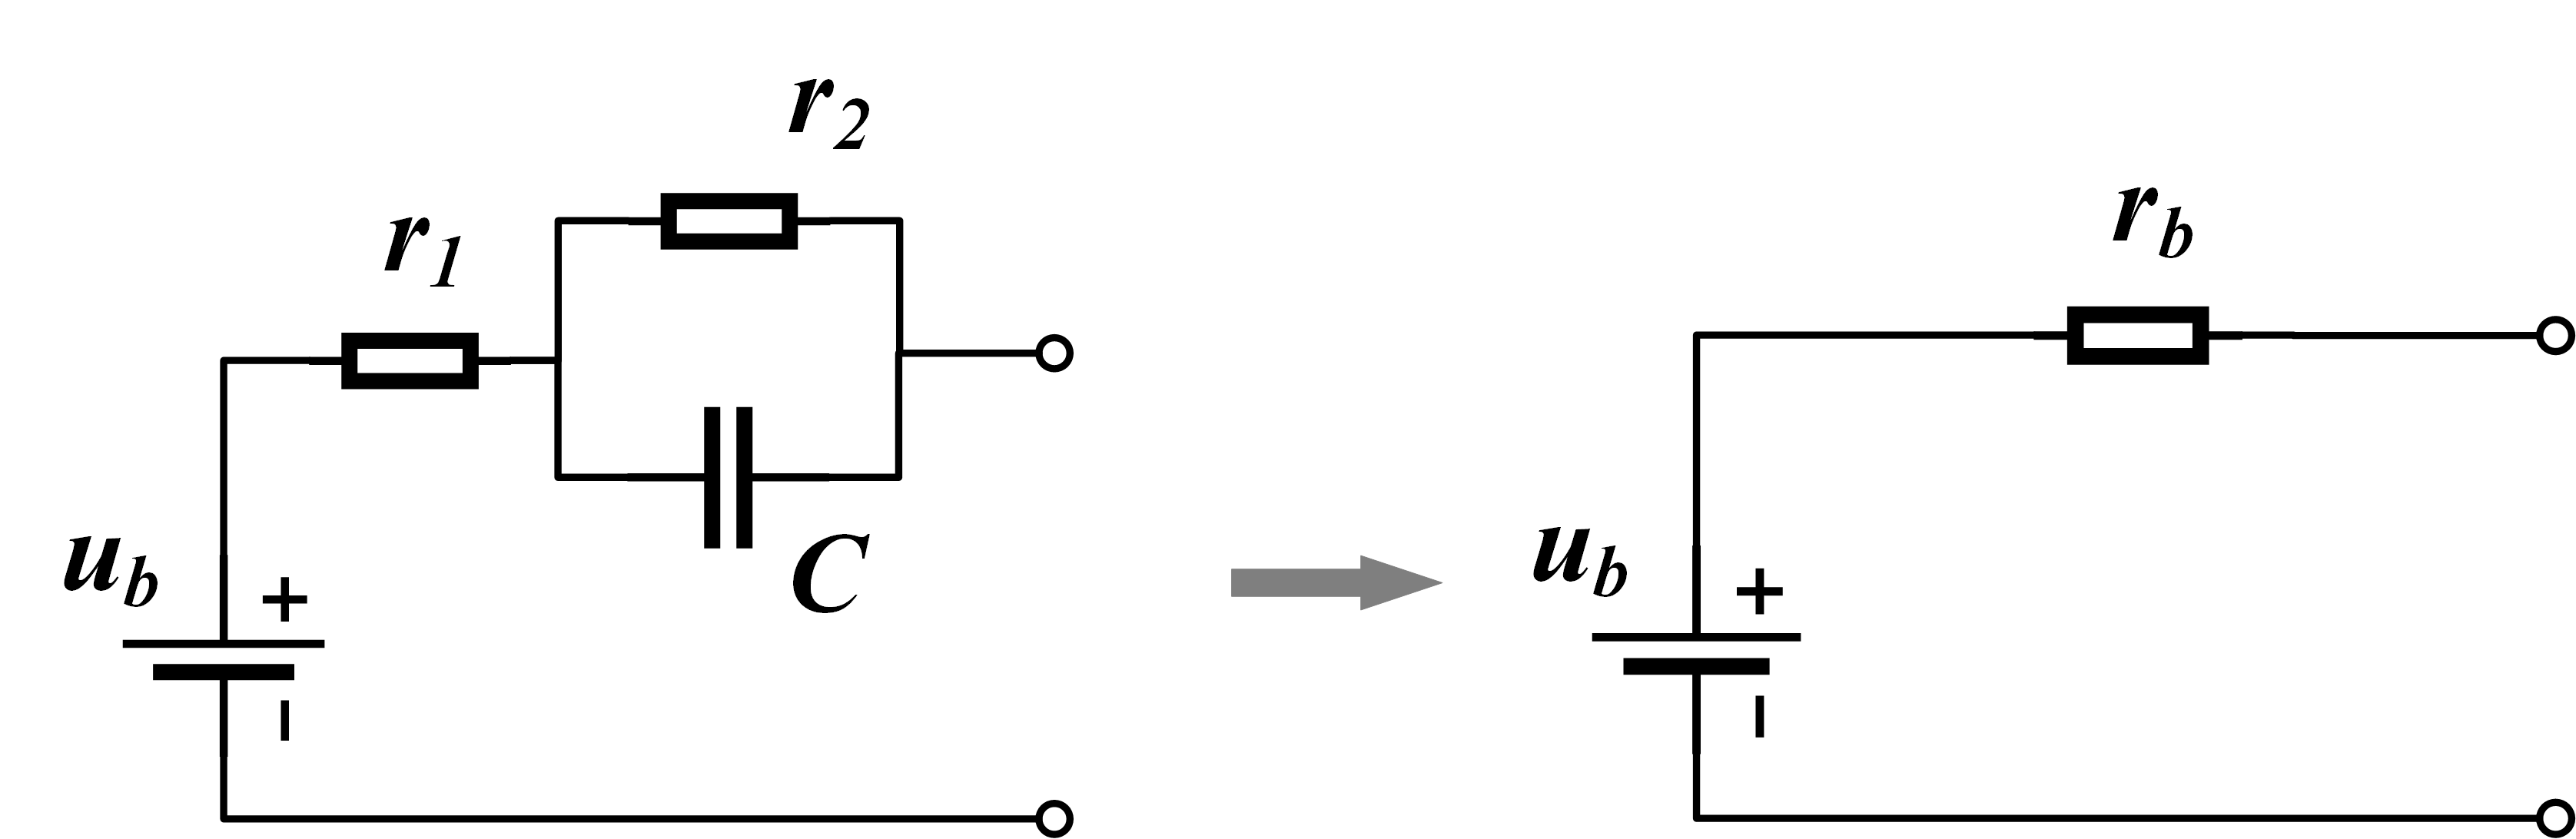
\includegraphics[width=0.8\linewidth]{battery_simple.png}
    }\label{fig:battery-simple}
    %\caption{
%        The directed graph models used in (a) the work of He et al. \cite{heExploringAdaptiveReconfiguration2013}, (b) our previous work, and (c) the improved model in this paper.
%        (d) The equivalent circuit of a battery in this method.
%    }
    \label{fig:model}
\end{figure}
\end{document}
